\documentclass[../main/main.tex]{subfiles}
\begin{document}

% \dominitoc
% \faketableofcontents
% \dominilof
% \fakelistoffigures
% \dominilot
% \fakelistoftables

\chapter{Variabilit\'es environnementales des SNe~Ia}\label{ch:env}

\epigraph{\openquote \textit{I like to think the moon is there even if I am not
looking at it.}\closequote}{Albert \textsc{Einstein}}

Dans le chapitre précédent, nous avons vu comment la physique des SNe~Ia
permettait de les utiliser comme des indicateurs de distance suffisamment précis
pour mesurer la quantité d'énergie noire de l'Univers (\textit{via} le paramètre
$w$), amenant à la découverte de son expansion accélérée. Les SNe~Ia permettent
également de mesurer le taux d'expansion actuel, nommé $H_0$, en se concentrant
sur la partie de bas redshift du diagramme de \textsc{Hubble}.

Avec l'augmentation rapide du nombre de SNe~Ia utilisables pour la cosmologie,
la mesure des paramètres cosmologiques ($H_0$ ou $w$ par exemple) commence à ne
plus être limitée par l'incertitude statistique mais par l'incertitude
systématique, c'est-à-dire par notre connaissance de leur physique intrinsèque
comme celle ayant permis leur standardisation. De nombreux efforts sont déployés
pour étudier la manière dont nous pouvons continuer à corriger les distances des
SNe~Ia avec d'autres paramètres.

Dans ce chapitre, nous présentons différents paramètres d'environnements
galactiques dans lesquels nous pouvons trouver des SNe~Ia
(Section~\ref{sec:envpres}) avant d'étudier la corrélation de leurs propriétés
avec les environnements les plus intéressants (Section~\ref{sec:envcorr}). De
cette Section découle notre travail de thèse.

\vfill
\minitoc
\vfill
\newpage

\section{Présentation d'environnements galactiques}\label{sec:envpres}

Dans le chapitre précédent, nous avons présenté les caractéristiques des SNe~Ia
en tant qu'objets individuels~; cependant, elles font la plupart du temps
partie d'un système bien plus large, les galaxies. Leur étude constitue un pan
entier de l'astrophysique et de la cosmologie, et nous n'avons pas prétention à
donner ici une zoologie complète de ce que sont les galaxies. Pour suivre le
déroulé de cette thèse, nous nous contentons de les décrire comme un ensemble
d'astres et de poussières en interaction gravitationnelle, pouvant comporter de
$10^8$ à $10^{14}$ étoiles et formant un tout dont le diamètre va de \num{1000}
à \SI{10000}{pc}.

Comme pour les SNe d'une manière générale (Ia, Ib…), il existe différents types
de galaxies et différentes caractéristiques décrivant des types
d'environnements, donnant toute une variété de formes, de couleurs et de
fonctionnements physiques. Nous présentons dans cette section quelques-unes de
ces caractéristiques galactiques.

\subsection{Morphologie}\label{ssec:morphost}

Au-delà de leur luminosité (qui est inhérente au fait d'être observé), l'aspect
visuel des galaxies est le premier facteur utilisé pour les classifier.
C'est~\cite{hubble1926} qui commence à les décrire en une classification qui
donnera plus tard \citep{hubble1936} le graphique présenté
Figure~\ref{fig:gmorph}, sobrement appelé «~séquence de \textsc{Hubble}~»,
depuis revisité et retravaillé. 

\begin{figure}[ht]
    \centering
    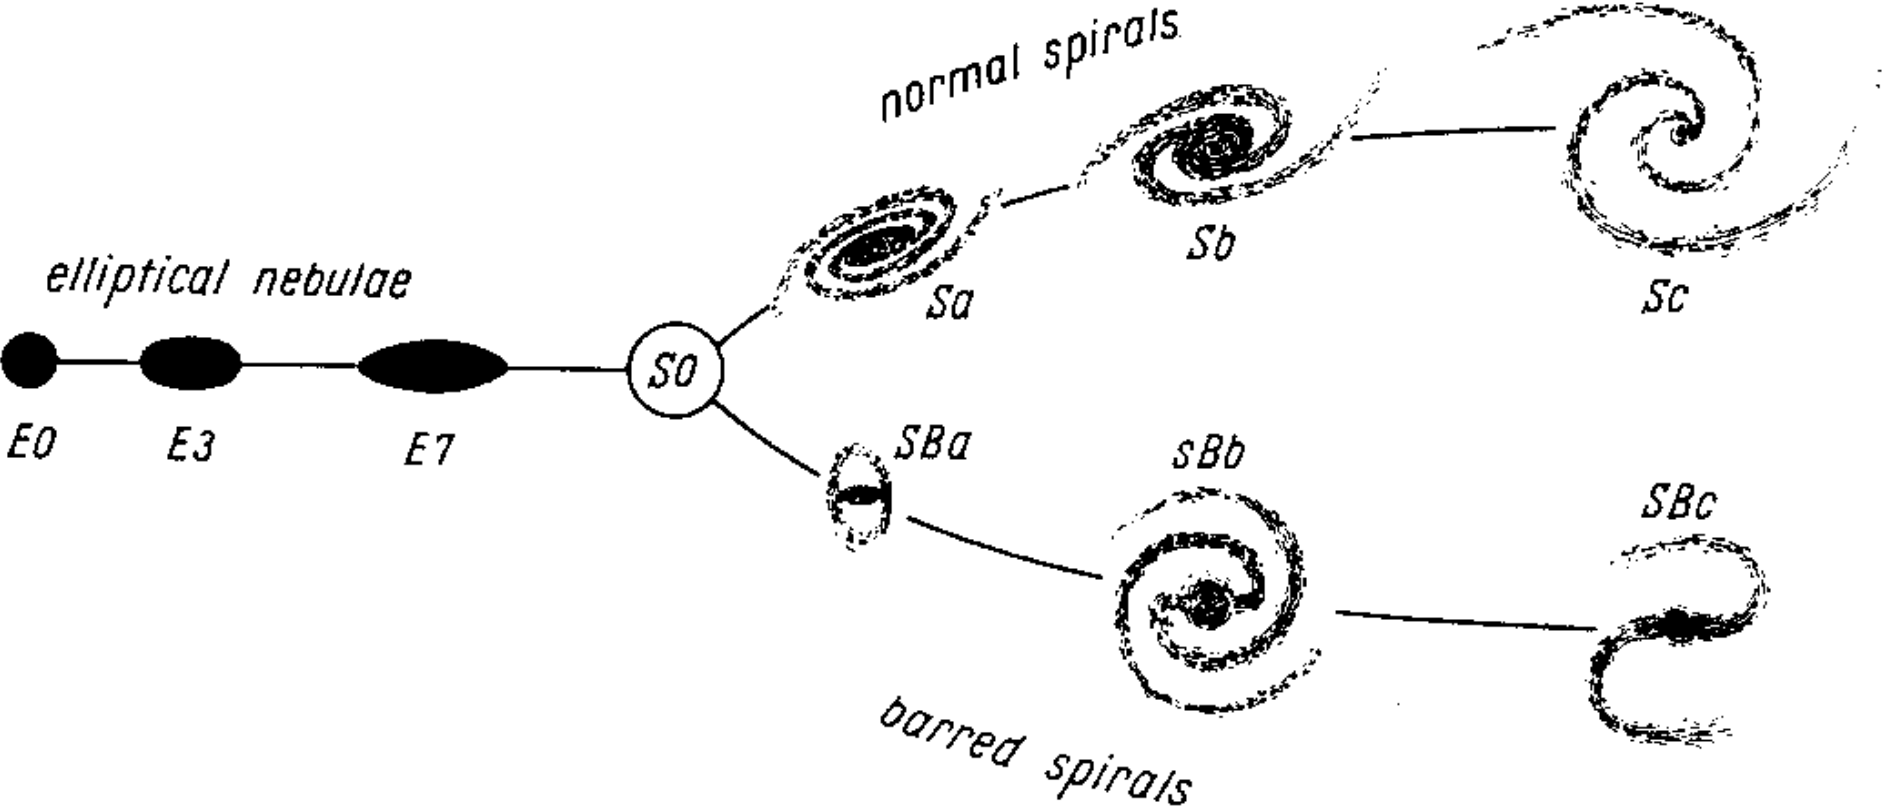
\includegraphics[width=\linewidth]{hubble_gmorph}
    \caption[Classification morphologique des galaxies]{Classification
        morphologique des galaxies d'après~\cite{hubble1936}. \textit{De gauche
        à droite}~: galaxies elliptiques (E0-7), lenticulaires (S0) et spirales,
    barrées \textit{en bas} (SBa-c) et non-barrées \textit{en haut} (Sa-c).}
    \label{fig:gmorph}
\end{figure}

Cette étude permet de rapporter trois grandes catégories de galaxies, illustrées
Figure~\ref{fig:gpict} par des images prises par le télescope spatial
\textsc{Hubble}\footnote{\label{fn:hst1}\href{
    https://www.nasa.gov/mission_pages/hubble/story/index.html}
{https://www.nasa.gov/mission\_pages/hubble/story/index.html}}~:

\begin{itemize}
    \item \textbf{Les elliptiques}, nommées par leur géométrie apparente,
        donnant lieu à des astres de luminosité continue\footnote{Donc sans
        sous-structure ou trou, mais cependant pas constante.} et diffuse sur
        leur surface. La classification va de E0 à E7 selon leur allongement, de
        sphérique à plate, respectivement~;
    \item \textbf{Les spirales}, présentant un bulbe central concentré en
        étoiles autour duquel tourne un disque s'arrangeant en bras spiralés.
        Elles sont distinguées selon la présence ou non-présence d'une barre
        (classifiées SB et S respectivement) semblant traverser le bulbe et
        duquel partent les bras. Elles se voient également sous-classifées
        «~a~», «~b~» ou «~c~» selon le rapport des surfaces entre le bulbe et le
        disque, de bulbe proéminent à bulbe peu marqué, respectivement~;
    \item \textbf{Les particulières}, regroupant toutes les autres morphologies
        ni tout à fait elliptiques ni tout à fait spirales~; par exemple les
        galaxies lenticulaires (S0 sur la Figure~\ref{fig:gmorph}), à mi-chemin
        entre les deux, les irrégulières (inclassables ou en interaction avec
        d'autres galaxies les déformant), etc.
\end{itemize}

\begin{figure}[t]
    \centering
    \begin{subfigure}[c]{.32\linewidth}
        \centering
        \includegraphics[height=5cm,
                         trim={4cm 7cm 2.5cm 4.5cm},
                         clip]{m87}
        \captionsetup{justification=centering}
        \caption{M87}
        \label{fig:m87}
    \end{subfigure}
    \hfill
    \begin{subfigure}[c]{.32\linewidth}
        \centering
        \includegraphics[height=5cm]{NGC3147}
        \captionsetup{justification=centering}
        \caption{NGC3147}
        \label{fig:ngc3147}
    \end{subfigure}
    \hfill
    \begin{subfigure}[c]{.32\linewidth}
        \centering
        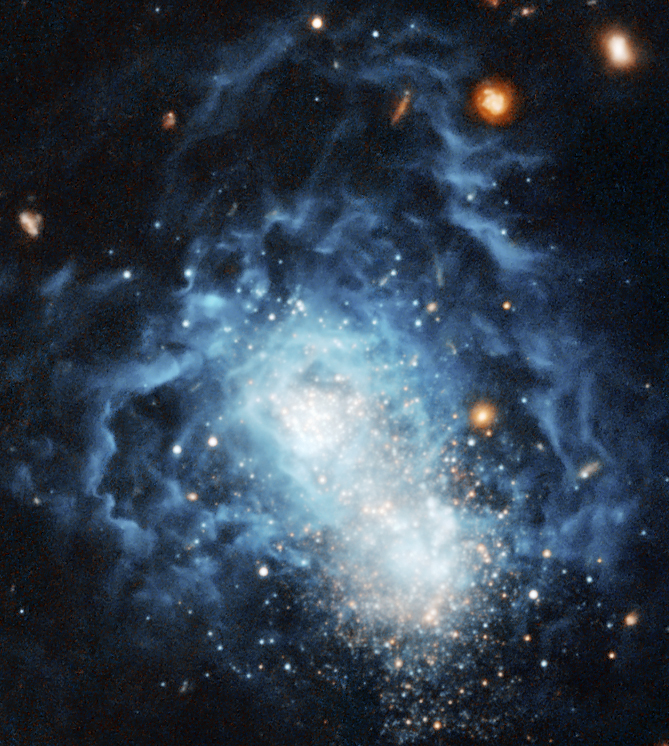
\includegraphics[height=5cm]{IZ18}
        \captionsetup{justification=centering}
        \caption{I Zw 18}
        \label{fig:iz18}
    \end{subfigure}
    \caption[Exemples de morphologies de galaxies]{Exemples de morphologies de
        galaxies. \textit{De gauche à droite}~: elliptique (M87), spirale
        (NGC3147) et irrégulière (I \textsc{Zwicky} 18). Images prises avec le
        télescope spatial \textsc{Hubble}\footnoteref{fn:hst1}, tirées
    du site \href{https://hubblesite.org}{hubblesite.org}.}
    \label{fig:gpict}
\end{figure}

Ce paramètre n'apparaît cependant pas comme un indicateur précis des propriétés
intrinsèques des SNe~Ia, comme nous le verrons par la suite.

\subsection{Couleur}\label{ssec:chost}

Comme pour les SNe~Ia (voir Section~\ref{ssec:lc}), nous pouvons caractériser la
couleur d'un environnement par une différence de magnitude entre deux bandes
photométriques. Cependant, ce paramètre est sujet à de nombreuses contaminations
extérieures~: dans un premier lieu, de la source à l'observation, le milieu
interstellaire présente un effet de rougissement qui peut être non-négligeable
selon la direction~; ensuite, la Voie Lactée peut ajouter une extinction
non-homogène selon les longueurs d'ondes~; finalement, l'atmosphère a elle aussi
un effet de rougissement selon son épaisseur et les conditions météorologiques
lors de la (ou des) mesures. En plus de cela, à cause de l'expansion de
l'Univers, les longueurs d'ondes subissent un décalage vers le rouge. Les
«~corrections $K$~» consistent à transposer les mesures pour les placer dans un
référentiel au repos, à $z=0$, ce qui permet des les corriger de cet effet et de
comparer les couleurs entre elles.

La multiplicité de ces possibles phénomènes parasites rend compliquées les
études utilisant la couleur comme mesure de l'environnement, mais font partie
intégrante des efforts de calibration pour la cosmologie observationnelle
\citep{fitzpatrick1999, schlafly2011, popovic2021b}.

\subsection{Masse stellaire}\label{ssec:mhost}

La masse stellaire $M_*$, exprimée en unité de masses solaires
(\si{\Msun})\footnote{Nous avons typiquement $10^{8}\si{\Msun} < M_* <
10^{12}\si{\Msun}$.}, constitue une autre caractéristique des galaxies. N'étant
pas une observable directe, elle se déduit par d'autres paramètres.
\cite{taylor2011} présentent une méthode de détermination de $M_*$ relativement
simple se basant sur la couleur des galaxies \textit{via} les magnitudes ($K$
corrigées) $g$ et $i$ des galaxies, telle que~:
\begin{equation}\label{eq:taylor}
    \log(M_* [\si{\Msun}]) = 1,16 + 0,70(g-i) -0,40 M_i
\end{equation}
avec $M_i$ la magnitude absolue de la galaxie dans la bande $i$. D'une manière
plus générale, celle-ci est déterminée par un ajustement de distributions
spectrales d'énergie\footnote{C'est-à-dire une mesure de flux lumineux en
fonction de la longueur d'onde.} (en anglais, \textit{spectral energy
distributions}, SED) générées à partir de modèles d'évolution stellaire (prenant
notamment en entrée une masse stellaire initiale et une paramétrisation de
l'historique de formation stellaire) avec la SED de la galaxie étudiée
\citep{walcher2011}.   Ce paramètre se trouve être un indicateur très utilisé en
cosmologie moderne, de par sa capacité à prédire d'autres caractéristiques des
galaxies.

% En supposant la quantité de vieilles étoiles proportionnelle à la masse
% stellaire $M_*$ de la galaxie hôte  Nous en voyons une utilisation pour les
% SNe~Ia dans la Section~\ref{sec:mcorr}.

\subsection{Taux de formation stellaire}\label{ssec:sfrhost}

En dehors de la masse à l'instant $t_0$ de l'observation, le taux de formation
stellaire (en anglais \textit{stellar formation rate}, SFR), exprimé en unité de
masses solaires formées par année (c'est-à-dire \si{\Msun.an^{-1}}), se trouve
être une caractéristique cruciale pour décrire les propriétés des étoiles d'une
galaxie. Son estimation se base sur l'émission de raies $H\alpha$, l'un des
indicateurs traditionnellement les plus utilisés pour mesurer le SFR
\citep{kennicutt1998}. Il repose sur le fait que les étoiles massives ($\gtrsim
\SI{20}{\Msun}$) génèrent des photons ultra-violets (donc à haute énergie)
capables d'ioniser les gaz d'hydrogène de leur environnement
\citep{calzetti2013} en grande quantité. Ces atomes excités vont ensuite se
recombiner, produisant diverses raies d'émission dont certaines dans la série de
\textsc{Balmer}, fournissant les raies $H\alpha$ dont la longueur d'onde dans le
vide est $\lambda_{H\alpha} = \SI{656.5}{nm}$. L'étude de cette raie permet
l'estimation de la formation stellaire du fait que les étoiles massives ont une
courte durée de vie, à l'échelle de millions d'années, et que leur capacité à
générer de tels photons ionisants décroît très rapidement~: le flux généré
décroît de deux ordres de grandeurs en approximativement \SI{10}{Mans}. La
présence d'hydrogène ionisé est donc un indicateur direct de la présence de
«~jeunes~» étoiles, c'est-à-dire de moins de \SI{100}{Mans}, et du taux de
formation stellaire \textit{via} la correspondance donnée
dans~\cite{calzetti2013}:
\begin{equation}\label{eq:sfrha}
    \mathrm{SFR}(H\alpha)\,[\si{\Msun.an^{-1}}] =
    5,45\times 10^{-42}L(H\a)\,[\si{erg.s^{-1}}]
\end{equation}
avec $L(H\alpha)$ la luminosité des raies d'émission, obtenue par un ajustement
spectral.

\subsection{Taux de formation stellaire spécifique
spectroscopique et âge}\label{ssec:lssfr}

Il est possible de tracer la fraction de jeunes étoiles \textit{via}
l'utilisation du taux de formation stellaire \textit{spécifique}, sSFR, tel
que~:
\begin{equation}\label{eq:ssfr}
    \mathrm{sSFR} = \frac{\mathrm{SFR}}{M_*}
\end{equation}
Nous l'appelons alors «~local~», et nous le dénotons LsSFR, quand ce ratio
calculé dans un environnement projeté de \SI{1}{kpc} autour de l'astre en
question. Cette approche locale a pour but de déterminer plus précisément l'âge
qu'avec des caractéristiques globales (morphologie, masse stellaire totale…).

\begin{figure}[t]
    \centering
    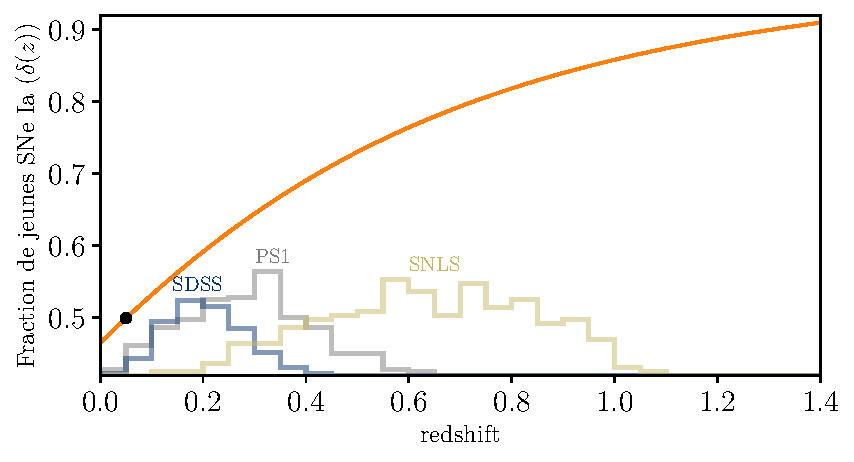
\includegraphics[width=.8\linewidth]{deltaz_hist}
    \caption[Évolution de la fraction de jeunes étoiles en fonction du
    redshift]{Évolution de la fraction de jeunes étoiles en fonction du
        redshift. La fraction est fixée à 50\% à $z=0,05$, représentée par le
        point noir. Les histogrammes représentent l'évolution du nombre de
        SNe~Ia relevées par différents sondages, montrant l'évolution de l'âge
    attendu des SNe à l'intérieur même des relevés.}
    \label{fig:deltaz}
\end{figure}

Il est attendu que la formation stellaire soit plus élevée à haut redshift (au
début de l'histoire de l'Univers) qu'à bas redshift, où les galaxies sont plus
vieilles et plus massives. Ainsi, le sSFR est un ordre de magnitude plus élevé à
$z = 1,5$ qu'à $z = 0$ \citep[voir][pour une étude complète]{madau2015}. En
pratique, les mesures de~\cite{tasca2015} trouvent un dépendance en redshift~:
\begin{equation}\label{eq:zssfr}
    \mathrm{sSFR} \propto (1+z)^{2,8 \pm 0,2}
\end{equation}
Les travaux de~\cite{rigault2020} combinent alors la fraction de jeunes étoiles
($\delta(z)$) et de vieilles étoiles ($\psi(z)$, telle que $\delta(z) + \psi(z)
= 1$) ainsi que l'équation~\ref{eq:zssfr} pour déduire~:
\begin{align}\label{eq:dpz}
    \mathrm{LsSFR}(z) \triangleq \frac{\delta(z)}{\psi(z)} &=
    K\times(1+z)^{\phi} \\\label{eq:deltaz}
    \text{et ainsi}\quad
    \delta(z) & = \left( K^{-1}\times(1+z)^{-\phi} +1 \right)^{-1}
    \\\label{eq:psiz}
    \psi(z)   & = \left( K\times(1+z)^{+\phi} +1 \right)^{-1}
\end{align}
avec $K=0,87$ en fixant $\delta(0,05) = \psi(0,05) = 0,5$ et $\phi = 2,8$. Nous
donnons Figure~\ref{fig:deltaz} une représentation graphique de l'évolution de
la fraction de jeunes étoiles en fonction du redshift.

\section{Corrélations des SNe~Ia à l'environnement}\label{sec:envcorr}

Ces indicateurs d'environnement peuvent être utilisés seuls ou conjointement
pour tenter de corréler les SNe~Ia à d'autres paramètres mesurables ou
estimables. Par exemple, il a été démontré que l'étirement d'une SN~Ia est
corrélé à la morphologie et à la masse de la galaxie hôte (voir
Figures~\ref{fig:x1gmorph} et~\ref{fig:mcorrx1}, respectivement).

\begin{figure}[ht]
    \centering
    \begin{subfigure}[c]{.48\linewidth}
        \centering
        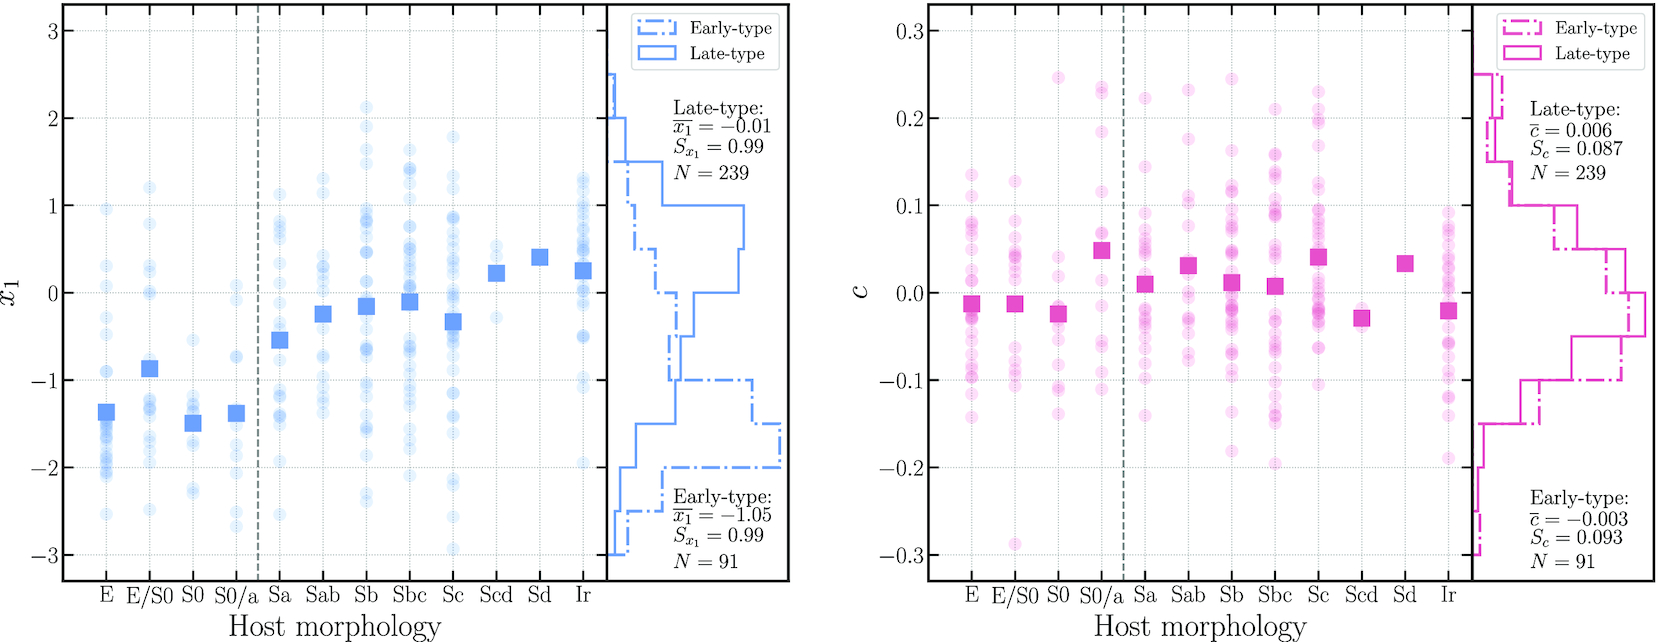
\includegraphics[height=5cm,
                         trim={0, 0, 6.665cm, 0},
                         clip]{x1gmorph}
        \caption[Corrélation entre l'étirement des SNe~Ia et la morphologie de
        leurs galaxies hôtes]{Corrélation entre l'étirement de 330 SNe~Ia de
            l'échantillon Pantheon \citep{scolnic2018} et la morphologie de
        leurs galaxies hôtes. Figure de~\cite{pruzhinskaya2020}.}
        \label{fig:x1gmorph}
    \end{subfigure}
    \hfill
    \begin{subfigure}[c]{.48\linewidth}
        \centering
        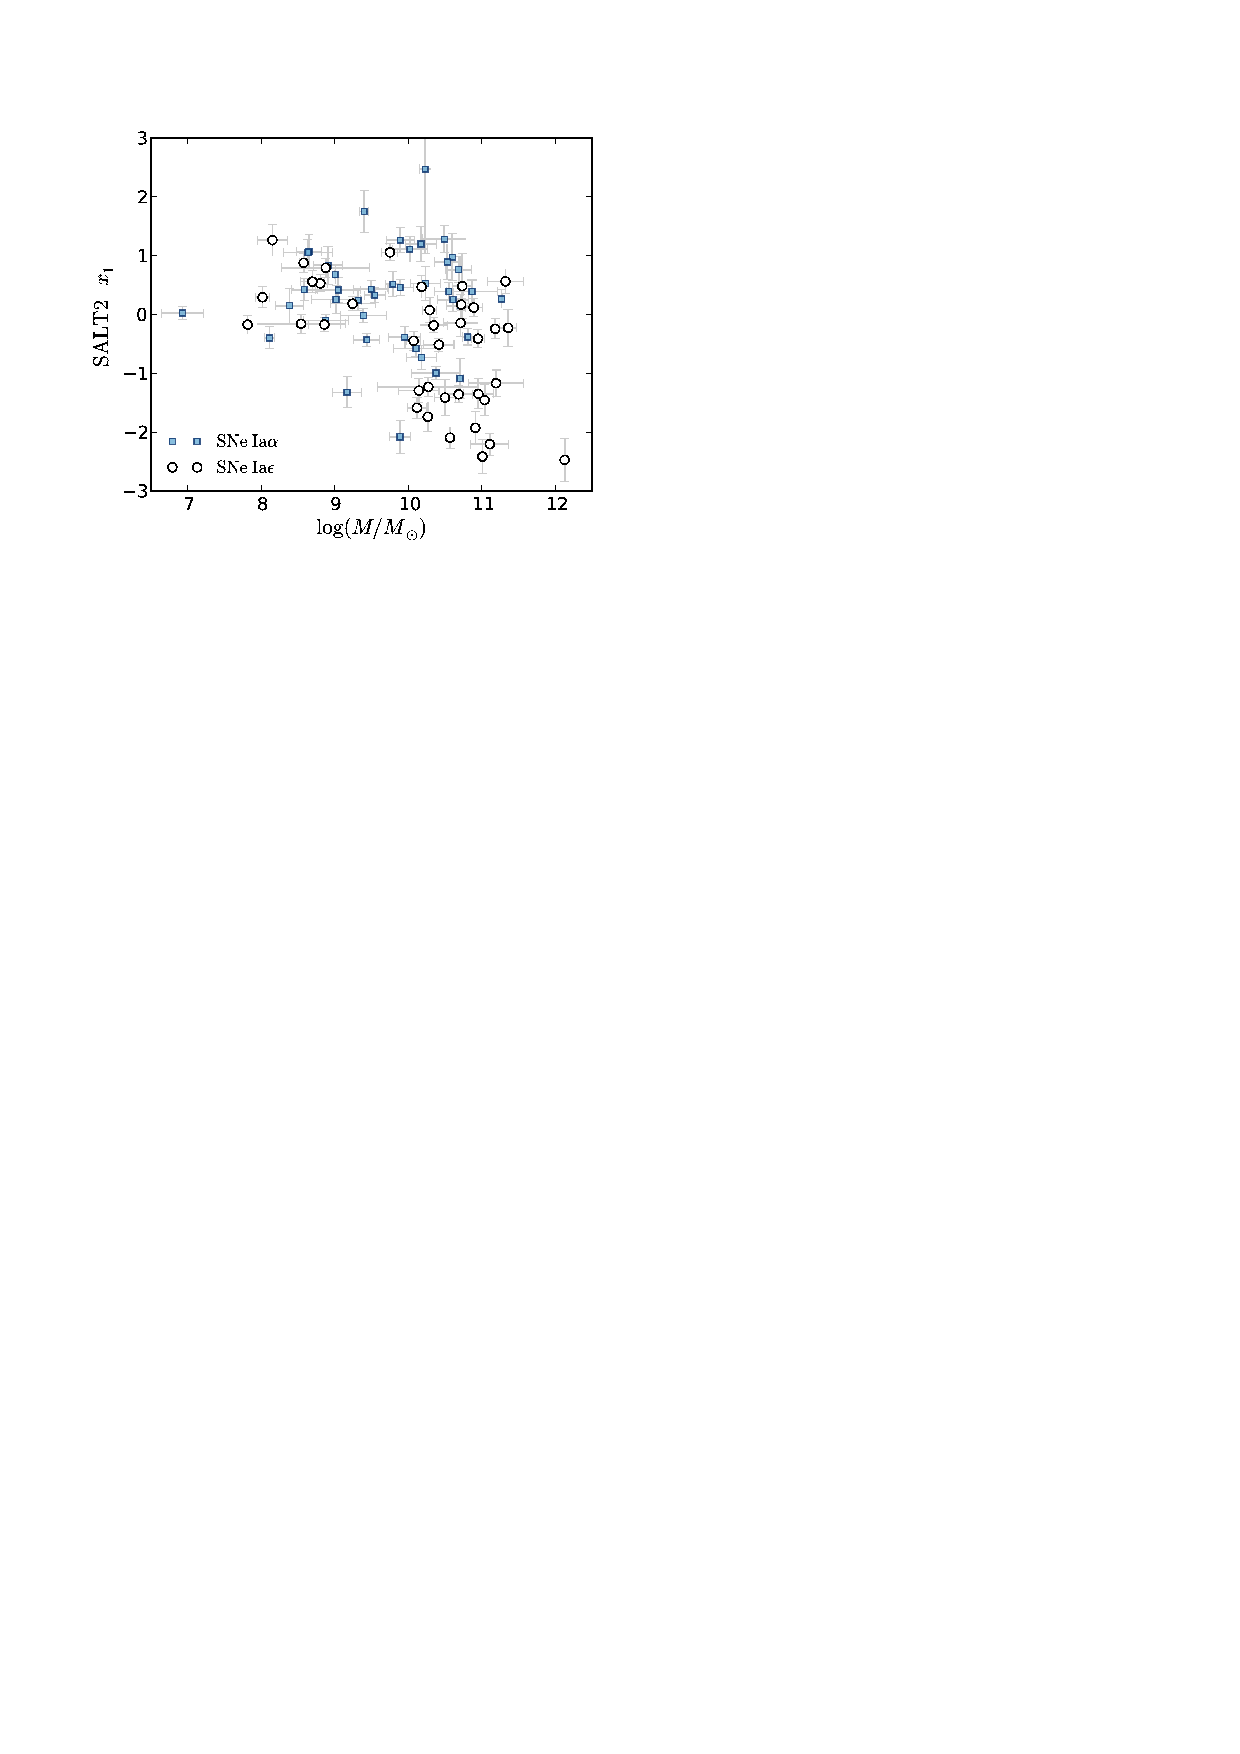
\includegraphics[height=5cm,
                         trim={1.5cm, 20.5cm, 10.5cm, 2.2cm},
                         clip]{rigault_x1vM}
        \caption[Corrélation entre l'étirement d'une SN et la masse de sa
        galaxie hôte]{Corrélation entre l'étirement d'une SN et la masse de sa
            galaxie hôte. La forme en «~L~» indique que ces distributions ne
        sont pas aléatoires. Figure de~\cite{rigault2013}.}
        \label{fig:mcorrx1}
    \end{subfigure}
    \caption[Corrélations entre l'étirement d'une SN~Ia et la morphologie ou la
    masse de sa galaxie hôte]{Corrélations entre l'étirement d'une SN~Ia et la
        morphologie (\textit{à gauche}) ou la masse de sa galaxie hôte
    (\textit{à droite})}
    \label{fig:x1corrs}
\end{figure}

De plus, \cite{mannucci2005, scannapieco2005, sullivan2006} avancent l'existence
de deux populations de SNe~Ia, dont le taux d'apparition de l'une serait
proportionnel à la masse stellaire globale et celui des secondes proportionnel
au taux de formation stellaire. Cette dichotomie de taux de SNe~Ia selon la
masse d'une part et le SFR d'autre part a lancé la notion d'âge de SNe~Ia,
partant d'abord de deux types~:
\begin{itemize}
    \item \textbf{Les promptes}~: elles sont associées à des étoiles
        relativement jeunes, entre \num{100} et \SI{500}{Mans}, de taux
        proportionnel au SFR~;
    \item \textbf{Les tardives}, associées à des étoiles vieilles, de plus de
        \SI{1}{Gans}, et de taux proportionnel à $M_*$.
\end{itemize}

Ainsi, \cite{rigault2020} stipule que le LsSFR serait également un traceur de
l'âge des SNe~Ia en plus de décrire l'évolution de la fraction de jeunes étoiles
avec le redshift. Une étude complète de la capacité de ce traceur à déterminer
l'âge d'une SNe~Ia a été effectuée dans~\cite{briday2021, briday2022}.

Cependant, afin d'améliorer la mesure des paramètres cosmologiques, il faut
avoir une correction sur leur luminosité qui elle-même améliore la mesure de
leurs distances \textit{via} l'équation de \textsc{Tripp}. À cet effet, de
multiples «~marches de magnitudes~» ont été implémentées dans les études
astrophysiques. Elles se basent sur une différence de luminosité entre deux
populations de SNe~Ia, discriminées par la valeur d'un paramètre. Nous
présentons dans cette section les marches de magnitudes basées sur la masse
(Section~\ref{ssec:mstep}) et sur l'âge (Section~\ref{ssec:astep}) avant de
motiver l'origine de notre thèse (Section~\ref{ssec:phdgoal}).

% Pour cela, l'idée de deux populations de SNe~Ia est prometteuse.

% \section{Corrélations avec la masse}\label{sec:mcorr}
% 
% Dans l'optique d'améliorer la précision de la mesure des paramètres
% cosmologiques avec les SNe~Ia, les efforts de standardisation ne cessent
% d'augmenter. À cet effet, la masse est apparue comme un indicateur permettant de
% réduire les incertitudes systématiques.
% 
% \subsection{Corrélation en étirement}\label{ssec:mcorrx1}
% 
% En étudiant les distributions d'étirement $x_1$ issus d'un ajustement par
% \texttt{SALT2.4}, de nombreuses études ont relevé une corrélation entre ce
% paramètre et la masse des galaxies hôtes des SNe~Ia testées \citep{neill2009,
% sullivan2010, rigault2013}. Ces études trouvent que les SNe~Ia dans les galaxies
% plus massives ont en moyenne un plus petit étirement que celles dans des
% galaxies moins massives. La distribution de ces deux paramètres donne une forme
% en «~L~», visible Figure~\ref{fig:mcorrx1}, et retrouvée bien plus tard dans
% cette thèse Figure~\ref{fig:2dhex}.

\subsection{Marche de magnitude basée sur la masse}\label{ssec:mstep}

% Cependant, tant que le coefficient $\alpha$ n'est pas affecté par une
% distribution autre, l'équation de \textsc{Tripp} ne sera pas modifiée et la
% correction appliquée aux SNe~Ia ne fournira pas de meilleure estimation de leur
% distance. Pour cela, il faut relier la luminosité des SNe~Ia avec leur
% environnement.

La première implémentation d'une correction de magnitude avec l'environnement
est celle basée sur la masse de la galaxie hôte. En effet, dès 2010 des études
ont observé une dépendance de la magnitude standardisée des SNe~Ia avec la masse
de leurs galaxies hôtes \citep[voir par exemple][]{kelly2010, betoule2014}. Nous
présentons Figure~\ref{fig:mbmass} un récent graphique de cette dépendance.

\begin{figure}[htb]
    \centering
    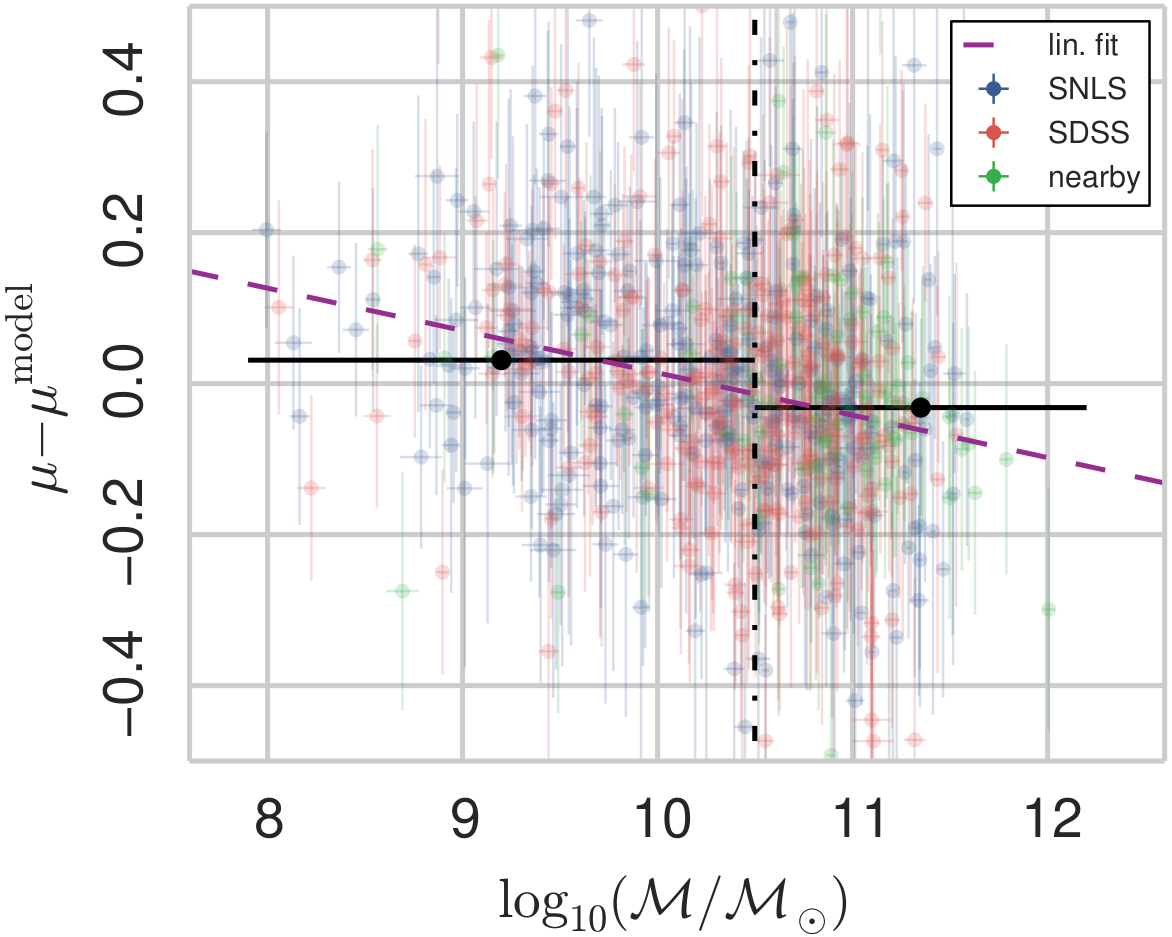
\includegraphics[width=.5\linewidth]{roman_ghub}
    \caption[Marche de magnitude basée sur la masse]{Différences entre les
        magnitudes corrigées des SNe~Ia et le modèle cosmologique de référence
        selon la masse de leurs galaxies hôtes. Nous observons que les SNe~Ia
        pour lesquelles $M_* < 10^{10}\Msun$ sont en moyenne moins lumineuses de
        +\SI{0.050}{mag} que celles de $M_* > 10^{10}\Msun$. Figure
    de~\cite{roman2018}.}
    \label{fig:mbmass}
\end{figure}

Dans ces études, il a été observé que les galaxies les plus
massives ($M_* > 10^{10}\si{\Msun}$) abritent des SNe~Ia en moyenne plus
lumineuses de $\gamma = -\SI{0.050}{mag}$ que celles ayant un hôte moins massif.
Cette corrélation se traduit par l'ajout d'un décalage en magnitude de
+\SI{0.025}{mag} pour les premières, et de -\SI{0.025}{mag} pour les secondes,
tel que~:
\begin{equation}\label{eq:mbmass}
    \mu = m_B - M + \alpha x_1 - \beta c \pm \gamma/2
\end{equation}

L'origine de cette corrélation reste cependant peu motivée autrement
qu'empiriquement. Cependant, comme présenté au début de la
Section~\ref{sec:envpres}, les galaxies sont des objets larges, et leurs
propriétés globales ne peuvent que partiellement décrire la physique de toutes
les SNe~Ia qui s'y trouveraient. 

\subsection{Marche de magnitude basée sur l'âge}\label{ssec:astep}

L'utilisation du LsSFR vise à réduire cette incertitude, en utilisant des
propriétés environnementales locales plutôt que globales. À cet effet,
\cite{rigault2020} rapportent une marche de magnitude basée sur l'âge de $\gamma
= \SI{0.16}{mag}$, dont nous présentons un graphique Figure~\ref{fig:rigahub}.

% \begin{figure}[ht]
%     \centering
%     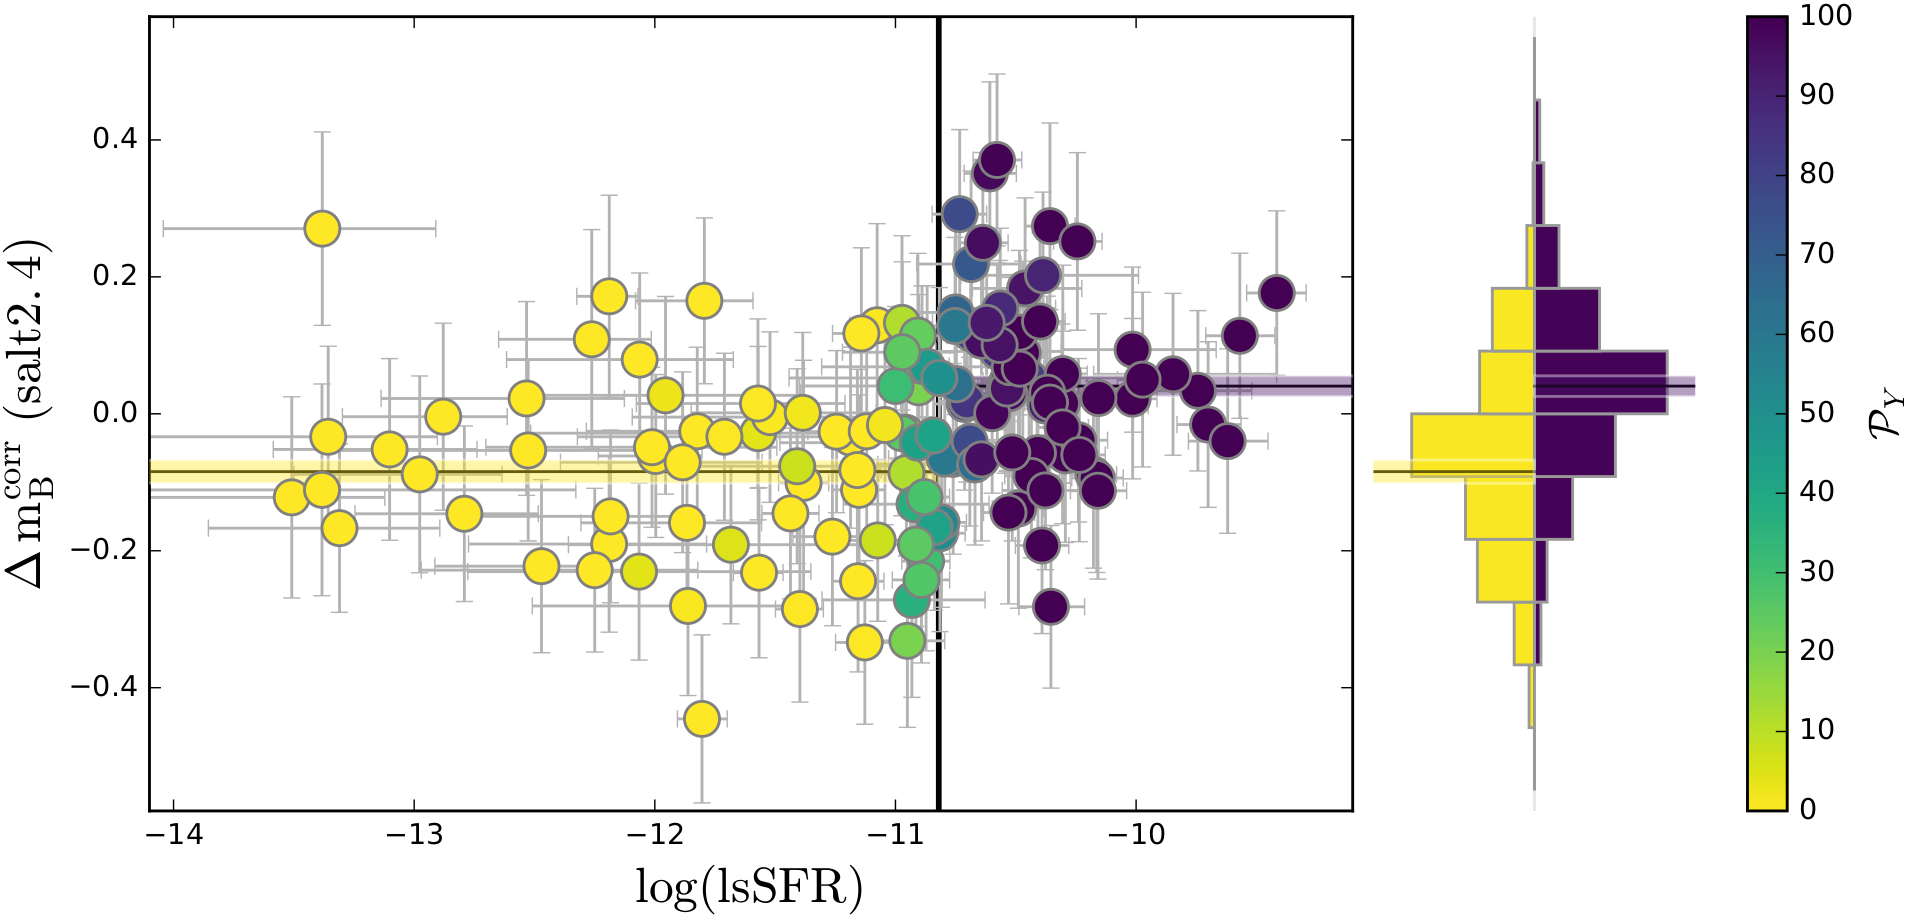
\includegraphics[width=.8\linewidth]{rigault_ahub}
%     \caption[Marche de magnitude basée sur l'âge]{\textit{Principal}~:
%         différences entre les magnitudes corrigées des SNe~Ia et le
%         modèle cosmologique de référence en fonction du LsSFR. \textit{Au
%         milieu}~: histogrammes pondérés par l'âge. Les lignes horizontales
%         représentent les moyennes des deux populations (et leurs erreurs).
%         Figure de~\cite{rigault2020}. Les couleurs correspondent à la
%         probabilité qu'une SN~Ia soit jeune, voir barre de couleur. Nous
%         observons que les SNe~Ia vieilles sont plus lumineuses de
%     -\SI{0.065}{mag} que les jeunes.}
%     \label{fig:rigahub}
% \end{figure}

\begin{figure}[ht]
    \centering
    \begin{subfigure}[c]{.48\linewidth}
        \centering
        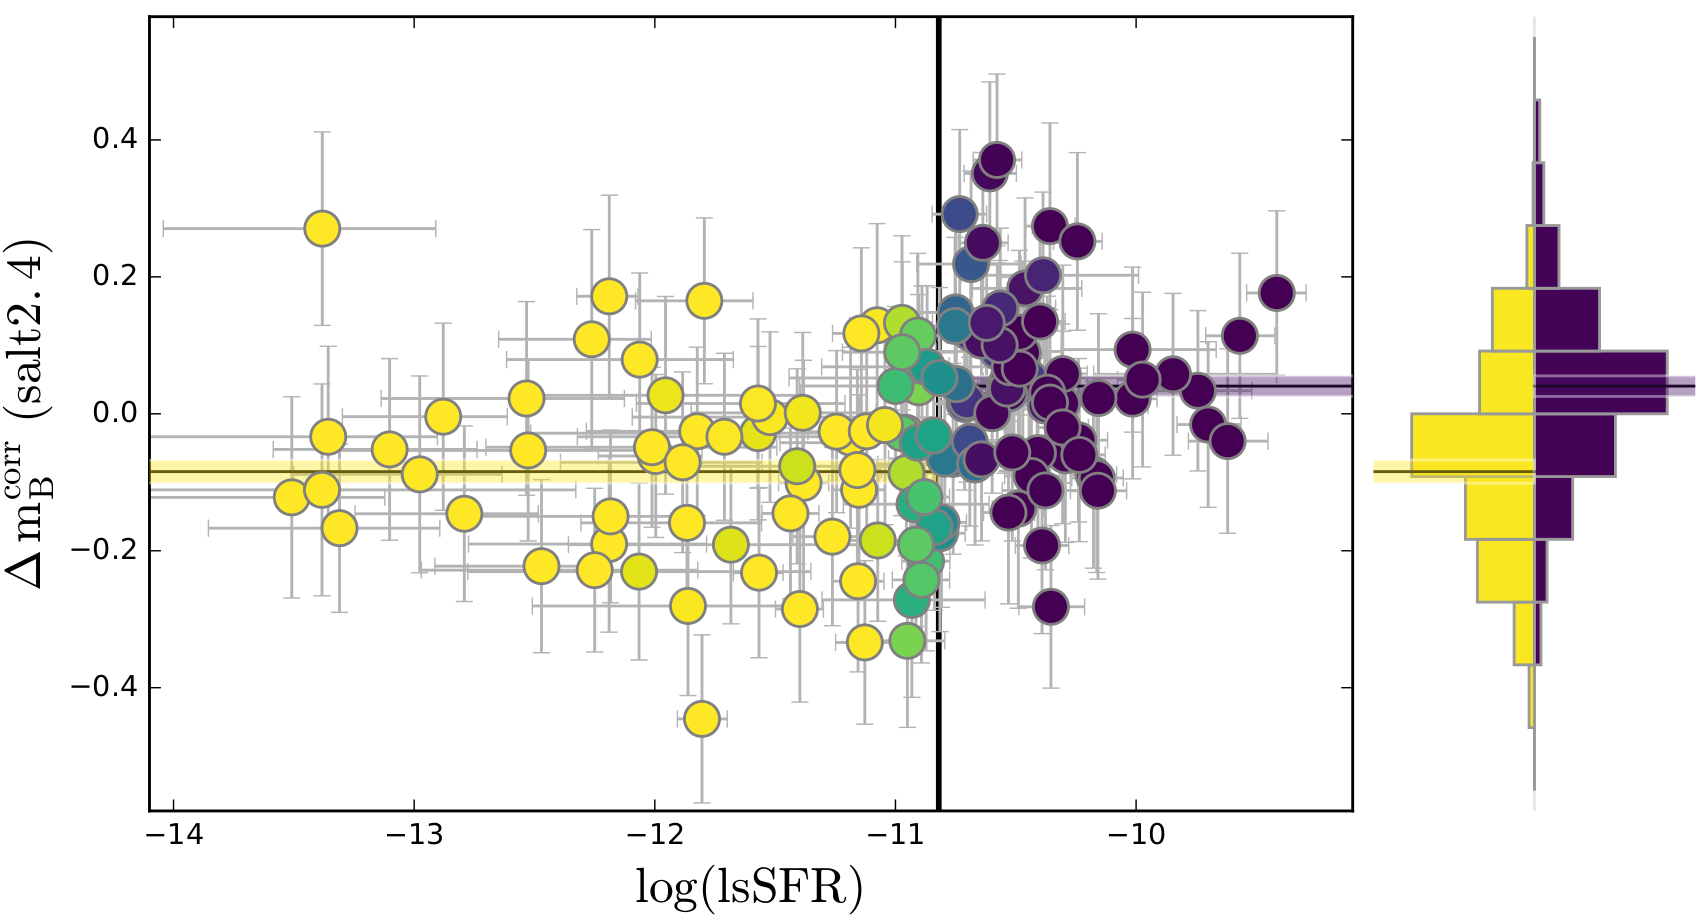
\includegraphics[height=4cm]{rigault_ahub-cut}
        \caption[Marche de magnitude basée sur l'âge]{Marche selon l'âge}
    \label{fig:rigahub}
    \end{subfigure}
    \begin{subfigure}[c]{.48\linewidth}
        \centering
        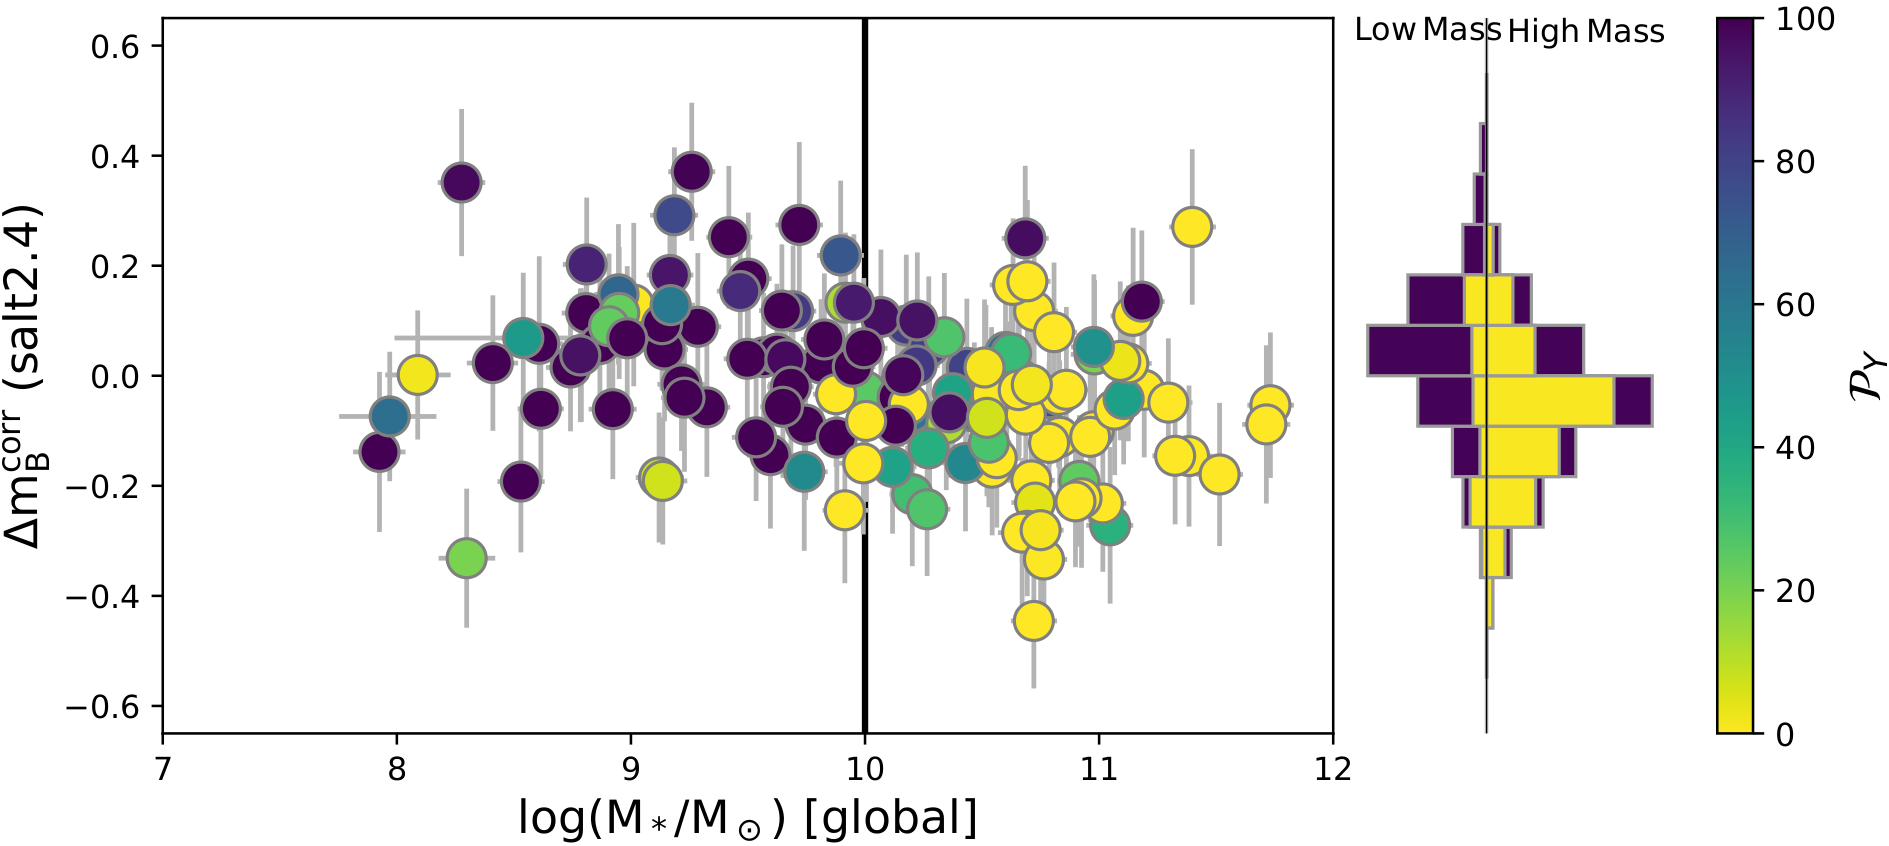
\includegraphics[height=4cm]{rigault_ghub}
        \caption[Marche de magnitude basée sur la masse]{Marche selon la masse}
    \label{fig:rigghub}
    \end{subfigure}
    \caption[Marches de magnitudes selon l'âge et la masse]{Marches de
        magnitudes selon l'âge (\textit{à gauche}) ou la masse (\textit{à
        droite}). Figures de~\cite{rigault2020}. Pour chacune des figures, nous
        avons en \textit{encadré} les différences entre les magnitudes corrigées
        des SNe~Ia et le modèle cosmologique de référence en fonction du
        paramètre concerné~; et \textit{à côté} les histogrammes pondérés par
        l'âge ou la masse. Les lignes horizontales représentent les moyennes des
        deux populations (et leurs erreurs). Les couleurs correspondent à la
        probabilité qu'une SN~Ia soit jeune, voir barre de couleur. Nous
        observons que les SNe~Ia vieilles sont plus lumineuses de
        -\SI{0.16}{mag} que les jeunes, alors que les SNe dans des
    environnements massifs ne le sont que de -\SI{0.12}{mag}.}
    \label{fig:rig}
\end{figure}

Cette approche de deux populations apporte une dimension supplémentaire à la
corrélation environnementale~: l'évolution avec le redshift. En effet, étant
donné que la fraction de jeunes étoiles évolue selon l'Équation~\ref{eq:deltaz},
la marche de magnitude moyenne varie avec le redshift, pouvant mener à des
estimations plus précises basées sur l'utilisation de paramètres plus pertinents
(car locaux). Nous notons notamment que~\cite{rigault2020} ont mesuré la marche
de magnitude trouvée en utilisant la masse des galaxies hôtes de leur
échantillons, et trouvent une différence proche d'autres
études~\citep{kelly2010, sullivan2010, gupta2011, childress2013} avec $\gamma =
\SI{0.12}{mag}$ comme le montre la Figure~\ref{fig:rigghub}. Cependant, les
auteurs rapportent des valeurs différentes quand l'ajustement des marches est
faite de manière conjointe~: les deux traceurs sont corrélés puisque le LsSFR
est relié à la masse de la galaxie hôte. Les valeurs sont alors
$\gamma_\text{âge} = \SI{0.13}{mag}$ et $\gamma{\rm masse} = \SI{0.06}{mag}$.
Cette étude montre la différence d'efficacité d'un paramètre à discriminer deux
populations et les conséquences que de telles différences causent sur la mesure
d'un même paramètre. Cette question est l'objet principal de la thèse
de~\cite{briday2021} qui a montré que le LsSFR se trouve être un meilleur
traceur des propriétés des SNe~Ia que les autres, réévaluant en même temps la
valeur attendue de marche basée sur l'âge à \SI{0.13}{mag}. C'est cette valeur
que nous utiliserons dans la suite.

\subsection{Implications en cosmologie moderne}\label{ssec:mcosmo}

Cette correction en fonction de la masse est actuellement utilisée pour corriger
les SNe~Ia qui sont utilisées dans la détermination de $H_0$. En effet, la
mesure directe de $H_0$ se base sur la mesure de distances avec les SNe~Ia,
comme nous avons pu le voir dans le Chapitre~\ref{ch:cosmo}, mais celle-ci doit
être calibrée en premier lieu. Pour cela, l'équipe \textit{Supernovae and
$H_0$ for the Equation of State of dark energy}~\citep[SH0ES,
Supernovae et $H_0$ pour l'équation d'état de l'énergie sombre][]{riess2021}
utilise des céphéides, de jeunes étoiles parmi les plus brillantes et dont la
magnitude absolue varie périodiquement. L'étude de cette loi magnitude-période
en permet la calibration et donc l'ancrage d'une première distance.

SH0ES applique cette étude pour des galaxies à la fois hôtes de céphéides et de
SNe~Ia, calibrant ainsi la distance des SNe~Ia en fonction de leur magnitude.
Cependant, l'environnement de ces galaxies est particulier, et est corrigée par
l'équipe en utilisant la standardisation en magnitude basée sur la masse~; ceci
augmente la valeur de $H_0$ de \SI{0.3}{km.s^{-1}.Mpc^{-1}} par rapport à une
absence de standardisation, pour une valeur finale de $H_0 =
\SI{73.04\pm1.04}{km.s^{-1}.Mpc^{-1}}$. Ce résultat, pourtant d'une qualité
d'étude irréfutable, est en désaccord à 5$\sigma$\footnote{C'est-à-dire qu'il
    n'y a qu'une chance sur 1 million que ces deux valeurs soient cohérentes et
que les mesures différentes soient le résultat d'une incertitude de calcul.}
avec la mesure indirecte du programme \textit{Planck}+$\Lambda$CDM
\citep{planck2018}, tout aussi irréfutablement précis, donnant $H_0 =
\SI{67.4\pm0.5}{km.s^{-1}.Mpc^{-1}}$. Cette tension est au cœur de
nombreuses discussions sur l'origine des différences.

L'utilisation de la marche de magnitude basée sur l'âge permet de réduire cette
incohérence étant donné que dans ces galaxies environ 95\% des environnements
sont jeunes. Ainsi, \cite{rigault2015} proposent l'utilisation de cette
corrélation âge-magnitude qui induirait sur la plus récente valeur une réduction
de \num{-1.94} sur la mesure directe, amenant la valeur à $H_0 =
\SI{71.10\pm1.04}{km.s^{-1}.Mpc^{-1}}$ et réduisant la tension. Cet exemple
permet de mesurer l'importance de la considération de l'environnement des SNe~Ia
dans leur correcte utilisation cosmologique.

\subsection{Ancrage de notre thèse~: étude de l'étirement en fonction de
l'âge}\label{ssec:phdgoal}

La mesure de caractéristiques des SNe~Ia en fonction de leur âge a également
amené~\cite{rigault2020} à étudier la distribution des étirements dans leur
échantillon. Cette étude révèle une dépendance de l'étirement en fonction de
l'âge des SNe~Ia, comme l'indique la Figure~\ref{fig:x1lssfr}, reproduite pour
cette thèse.

\begin{figure}[ht]
    \centering
    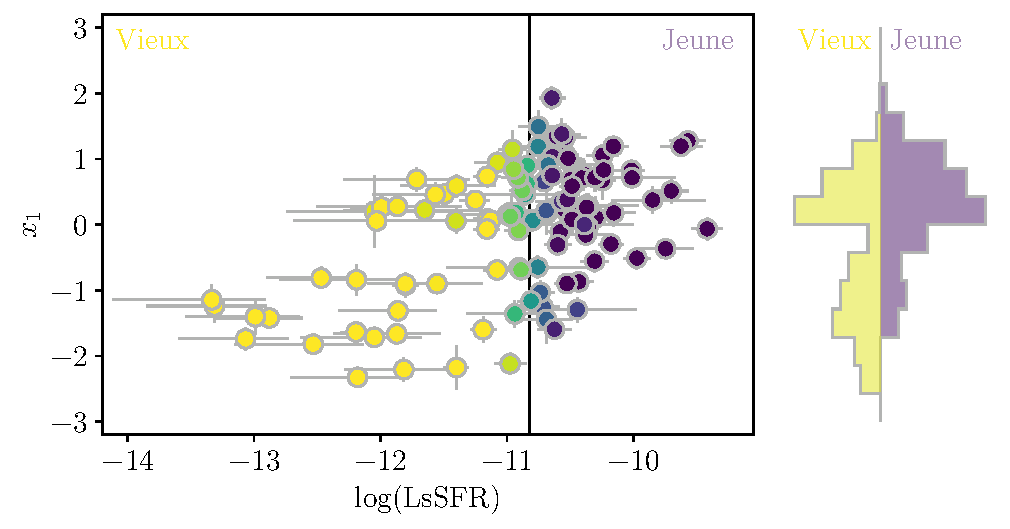
\includegraphics[width=.8\linewidth]{model_base_hist-nomodel}
    \caption[Dispersion de l'étirement en fonction du LsSFR]{\textit{Principal}:
        étirement de courbe de lumière ($x_1$) issu d'un ajustement par
        \textsc{\texttt{SALT2.4}} en fonction du LsSFR pour certaines SNe
        de~\cite{rigault2020}, figure reproduite. La couleur correspond à la
        probabilité $p_y$ que la SN~Ia soit jeune, voir Figure~\ref{fig:rig}.
        \textit{À droite}: histogramme pondéré par $p_y$ des étirements des SNe.
        Les contributions de la population jeune et âgée sont indiquées en
    violet et en jaune, respectivement.}
    \label{fig:x1lssfr}
\end{figure}

Cette étude permet d'augmenter l'étude du LsSFR comme traceur correct des
propriétés intrinsèques des SNe~Ia en mettant en lumière la possible existence
de distributions sous-jacentes d'étirement différentes selon l'âge d'une SN~Ia,
et donc appuyer l'existence de deux populations de SNe~Ia qui seraient le mieux
discriminées par l'âge. En effet, l'histogramme de la Figure~\ref{fig:x1lssfr}
laisse à penser que les SNe~Ia vieilles sont distribuées différemment des
jeunes, présentant un pic de probabilité fort à $x_1 \approx -1$.

Comme nous l'avons vu au début de la Section~\ref{sec:envcorr}, une telle
corrélation est intéressante mais n'impactera pas directement la détermination
des distances des SNe~Ia, n'agissant pas directement sur la magnitude.
Cependant, comme pour la marche de magnitude basée sur l'âge, la fraction de
jeunes étoiles varie avec le redshift selon l'Équation~\ref{eq:deltaz}, et avec
elle l'importance d'une distribution d'étirement par rapport à l'autre. Nous
pourrions ainsi déterminer l'évolution de la distribution de l'étirement des
SNe~Ia en fonction du redshift. Ce phénomène n'est, à notre connaissance, pas
étudié sous cette forme à ce jour mais joue pourtant un rôle important dans les
simulations numériques de SNe~Ia, celles-ci utilisant des distributions de
probabilité desquelles tirer des valeurs d'étirement pour reproduire ce que les
sondages observent.

C'est dans ce contexte que s'ancre notre thèse. Afin de réaliser cette étude,
nous allons présenter les sondages dont nous allons utiliser les données
(Chapitre~\ref{ch:surveys}) afin de constituer un échantillon correspondant à
nos restrictions (Chapitre~\ref{ch:sample})~; celui-ci sera utilisé pour
déterminer la possible évolution de l'étirement avec le redshift
(Chapitre~\ref{ch:stretch}). Le modèle qui en découle sera injecté dans un
programme de simulation (Chapitre~\ref{ch:snana}) qui nous permettra de sonder
le biais attendu sur la valeur de $w$ si cette dépendance environnementale est
incorrectement prise en compte dans les études sur les paramètres cosmologiques
(Chapitre~\ref{ch:sims}).

\clearpage

\thispagestyle{plain}
% \vspace*{-3cm}
\vfill
\minilof
\vfill
\minilot
\vfill

% \bibliographystyle{../main/aa_url}
% \shorthandoff{:}
% \bibliography{../chapters/99_references}

\end{document}
